\documentclass[conference]{IEEEtran}
\usepackage[T1]{fontenc}
\usepackage[utf8]{inputenc}
\usepackage{amsmath}
\usepackage{amsfonts}
\usepackage{amssymb}
\usepackage{graphicx}
\usepackage[left=1cm, right=1cm, top=1cm, bottom=1cm]{geometry}
\usepackage{float} % For [H] placement of figures
\usepackage{hyperref} % For clickable links and references
\usepackage{listings} % For code snippets
\usepackage{xcolor} % For coloring code
\usepackage{subcaption}

\title{Hybrid AI for Intelligent Street Lighting: Regression, Fuzzy Reasoning, and Evolutionary Tuning}
\author{
\IEEEauthorblockN{(Everyone has done equal amount of work) \\ Michał Mazurek, Marcin Basisty, Łukasz Święch, Byeongjun Min}
\IEEEauthorblockA{
Faculty of Physics and Applied Computer Science\\
AGH University of Science\\
Krakow, Poland\\
}
}

\begin{document}

\maketitle
\begin{abstract}
Urban street lighting is essential for safety and mobility, yet conventional systems are often inefficient, static, or reactive, wasting energy and sometimes failing to provide adequate illumination during critical periods. Rapidly changing pedestrian activity, traffic flow, and environmental conditions demand a smarter approach that can balance safety and sustainability.

This work introduces a hybrid artificial intelligence framework for adaptive street lighting that combines predictive modeling, interpretable reasoning, and evolutionary optimization. A regression-based predictor anticipates short-term lighting needs using real-time sensor data and contextual information from the IoT-enabled smart lighting dataset \cite{smartlighting_dataset}, while a fuzzy-rule-based layer embeds expert knowledge to ensure safe illumination under uncertain or extreme conditions. System parameters, including fuzzy membership functions and control thresholds, are optimized using a multi-objective evolutionary algorithm to produce Pareto-optimal solutions balancing energy efficiency and predicted safety risk.

Evaluation on the Kaggle IoT dataset demonstrates that the hybrid system significantly reduces energy consumption while maintaining high safety standards, outperforming static schedules and purely data-driven strategies. By integrating prediction, expert reasoning, and optimization, this approach delivers an intelligent, transparent, and resilient solution for smart city street lighting, enabling sustainable and context-aware urban illumination.
\end{abstract}

\section{Introduction}

Street lighting is a fundamental element of urban infrastructure, crucial for road safety, pedestrian security, and overall quality of life. Yet conventional lighting systems typically operate on static schedules or simple threshold rules, resulting in unnecessary energy use during periods of low activity and occasionally insufficient illumination when demand spikes. As cities seek to reduce energy consumption and meet sustainability goals, there is a growing need for lighting systems that can adapt intelligently to dynamic urban conditions.

The increase of IoT sensors and smart city technologies now enables continuous monitoring of environmental and activity data, including ambient light, weather, pedestrian flow, vehicle traffic, and historical energy usage. While these rich data streams open the door to intelligent control, they also introduce complexity, noise, and uncertainty that challenge traditional rule-based strategies.

Machine learning (ML) offers the ability to model nonlinear relationships between context and lighting demand, but purely data-driven approaches often lack transparency and can behave unpredictably under unseen or noisy conditions. In safety-critical public infrastructure, such opacity limits trust and deployability.

Hybrid AI approaches address these challenges by combining predictive intelligence with interpretable reasoning. Fuzzy logic, in particular, provides human-readable decision rules that can enforce safe, conservative behavior under uncertainty. Integrating fuzzy reasoning with ML predictions stabilizes control outputs while explicitly incorporating domain knowledge.

In this work, we present a hybrid smart street lighting framework that unites ML-based demand estimation, fuzzy-rule-based reasoning, and multi-objective evolutionary optimization. The approach adapts illumination dynamically to activity and environmental conditions, optimizes energy use, and maintains safety. Subsequent sections detail the dataset, modeling methodology, fuzzy system design, optimization strategy, evaluation protocol, and experimental results demonstrating the system’s effectiveness.

\subsection{Dataset Description and Preprocessing}
The experiments use the IoT-enabled smart lighting dataset from Kaggle \cite{smartlighting_dataset}, which contains sensor measurements from multiple urban zones, capturing environmental, occupancy, and energy-related features relevant to adaptive street lighting. The target variable for supervised learning is the adjusted lighting output, \texttt{adjusted\_light\_intensity}, representing the effective lighting level selected under the observed conditions.

\subsection{Safety Risk Score Calculation}
We create a new feature called \texttt{safety\_risk\_score}, which enables capturing the combined effect of pedestrian activity, traffic conditions, and contextual events as a unified safety metric.

The base safety risk score is defined as a weighted linear combination:
\begin{equation}
R_{\text{base}} = 0.15 \cdot M + 0.35 \cdot O + 0.35 \cdot T + 0.15 \cdot S
\end{equation}
where $M$ denotes motion detection, $O$ normalized occupancy count, $T$ normalized traffic density, and $S$ normalized pedestrian speed. The weights are chosen heuristically to emphasize real-time activity and crowd presence.

To account for atypical conditions such as public events, the score is amplified when the \texttt{special\_event\_flag} is active:
\begin{equation}
R_{\text{safety}} = R_{\text{base}} \cdot (1 + \alpha E),
\end{equation}
where $E \in \{0,1\}$ indicates a special event and $\alpha = 0.30$. The final score is clipped to $[0,1]$ and added to the dataset.

\subsection{Correlation Heatmap}

The heatmap reveals several key relationships in the numerical features. Notably, \texttt{motion\_detected} and \texttt{safety\_risk\_score} exhibit a near-perfect positive correlation of 0.95, indicating that detected movement is the primary driver of the safety assessment. Additionally, \texttt{adjusted\_light\_intensity} is strongly correlated with \texttt{energy\_consumption\_kwh} ($r=0.92$) and inversely correlated with \texttt{ambient\_light\_lux} ($r=-0.52$), reflecting efficient dimming under natural illumination. Human activity metrics, such as \texttt{occupancy\_count} and \texttt{traffic\_density} ($r=0.61$), serve as secondary but meaningful predictors of both energy demand and the computed safety score.

\begin{figure}[H]
\centering
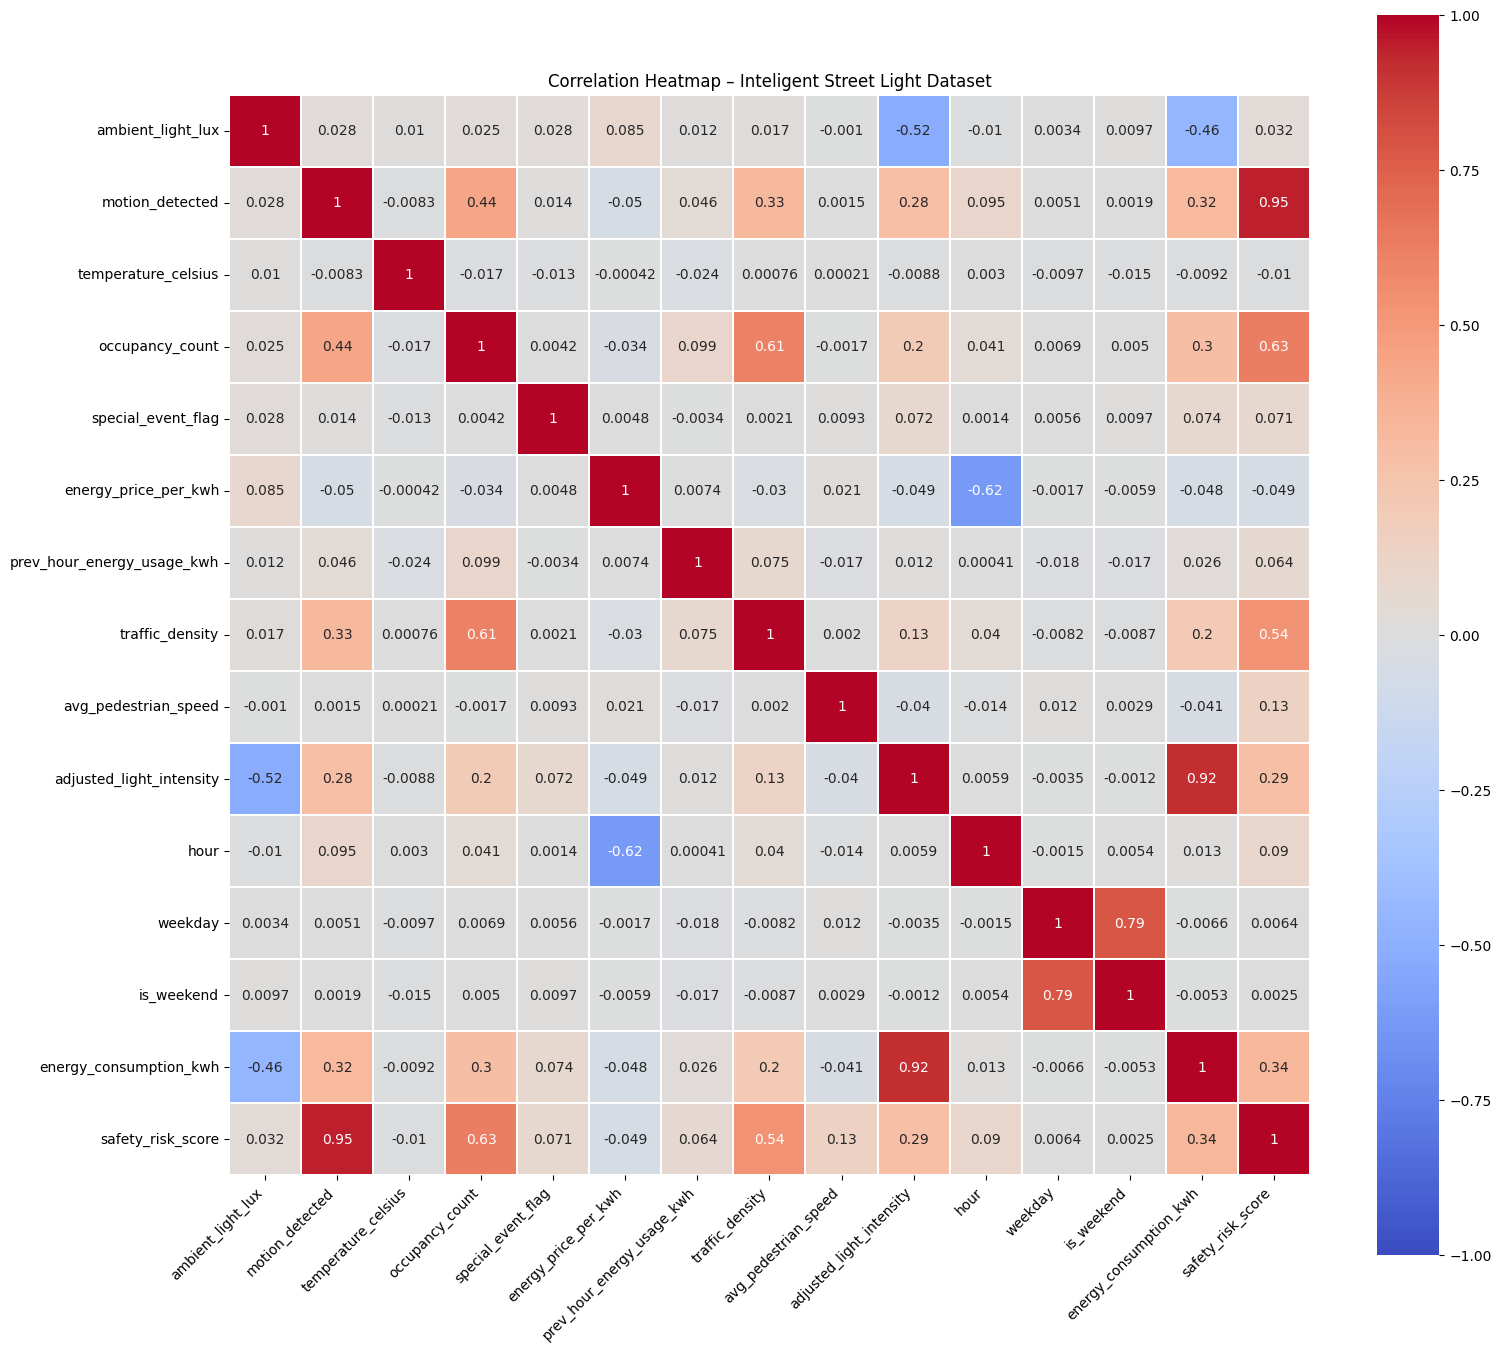
\includegraphics[width=0.4\textwidth]{assets/CorrMatrix.png}
\caption{Correlation heatmap of key numerical features, highlighting relationships between ambient light, occupancy count, motion detection, and energy usage.}
\label{fig:heatmap}
\end{figure}

\section{Fuzzy Logic System for Adaptive Lighting Control}
The primary motivation was to introduce human-like reasoning into the decision-making process for adjusting light intensity, particularly in situations where the MLP's predictions might deviate significantly from expected behavior or when environmental factors involve a rule-based adjustment.

The fuzzy inference system uses two input variables and one output variable, all normalized to the range $[0,1]$.

\begin{itemize}
    \item \textbf{Activity Level}: Represents the level of human or vehicle presence in a lighting zone. It is derived from \texttt{occupancy\_count}, where higher values indicate greater activity. Three triangular membership functions are defined to describe the linguistic terms \emph{low}, \emph{medium}, and \emph{high}.
    
    \item \textbf{Visibility Level}: Captures environmental factors affecting visibility, including ambient light and temporal context.

    \item \textbf{Lighting Intensity}: This is the output variable of the fuzzy system and represents the recommended lighting level. It is described using three linguistic terms: \emph{dim}, \emph{normal}, and \emph{full}.
\end{itemize}

The fuzzy rule base defines how lighting intensity should be adjusted based on activity and visibility levels. A total of nine rules were designed to cover all meaningful combinations of these inputs.

\section{Multi-Objective Differential Evolution with Sobol Initialization}

Lighting control parameters are optimized using a multi-objective Differential Evolution (DE) algorithm with Sobol low-discrepancy sequences, simultaneously minimizing energy consumption and predicted safety violations.

The initial population is generated as
\begin{equation}
\mathbf{x}_i = \mathbf{l} + (\mathbf{u} - \mathbf{l}) \odot \mathbf{s}_i,
\end{equation}
where $\mathbf{s}_i \in [0,1]^D$ denotes a Sobol sample and $\mathbf{l}, \mathbf{u}$ are decision bounds.

Each candidate solution represents lighting intensity levels over discrete time blocks and is evaluated using a bi-objective formulation:
\begin{equation}
\min_{\mathbf{x}} \; \mathbf{f}(\mathbf{x}) = \left( f_1(\mathbf{x}), f_2(\mathbf{x}) \right).
\end{equation}

The first objective measures average energy consumption:
\begin{equation}
f_1(\mathbf{x}) = \frac{1}{N} \sum_{i=1}^{N} P_{\max} \cdot \frac{x_{h_i}}{100} \cdot \Delta t_i,
\end{equation}
while the second minimizes predicted safety violations using a trained MLP:
\begin{equation}
f_2(\mathbf{x}) = \frac{1}{N} \sum_{i=1}^{N} \hat{v}_i(\mathbf{x}).
\end{equation}

The DE/rand/1/bin strategy is employed, with mutation defined as
\begin{equation}
\mathbf{v}_i = \mathbf{x}_{r_1} + F(\mathbf{x}_{r_2} - \mathbf{x}_{r_3}),
\end{equation}
followed by binomial crossover and boundary clipping. Selection is based on Pareto dominance, and after a fixed number of generations, the non-dominated solutions form an approximation of the Pareto front:
\begin{equation}
\mathcal{P} = \left\{ \mathbf{x}_i \mid \nexists \mathbf{x}_j : \mathbf{f}(\mathbf{x}_j) \prec \mathbf{f}(\mathbf{x}_i) \right\}.
\end{equation}

\subsection{Outcome}

The extracted Pareto-optimal solutions characterize the trade-off between energy efficiency and safety performance. By integrating Sobol initialization with Pareto-based selection, the proposed approach achieves improved convergence robustness and maintains solution diversity relative to conventional randomly initialized or single-objective DE methods.

\section{Exploratory Data Analysis and Feature Relationships}
To better understand the structure of the dataset and the relationships between key features, several visualizations were created. These plots provide insight into patterns of energy consumption, pedestrian and traffic activity, environmental conditions, and safety considerations.

\subsection{Energy Consumption Patterns}
Mean hourly energy consumption was analysed to identify temporal trends in street lighting demand. As expected, energy usage peaks during evening hours and decreases during low-activity periods, such as early morning. 

Energy consumption was also examined with respect to weather conditions. Results indicate that adverse conditions, such as rain or fog, lead to higher energy usage, reflecting increased lighting needs for visibility and safety.

\begin{figure}[H]
    \centering
    \begin{subfigure}[b]{0.48\linewidth} 
        \centering
        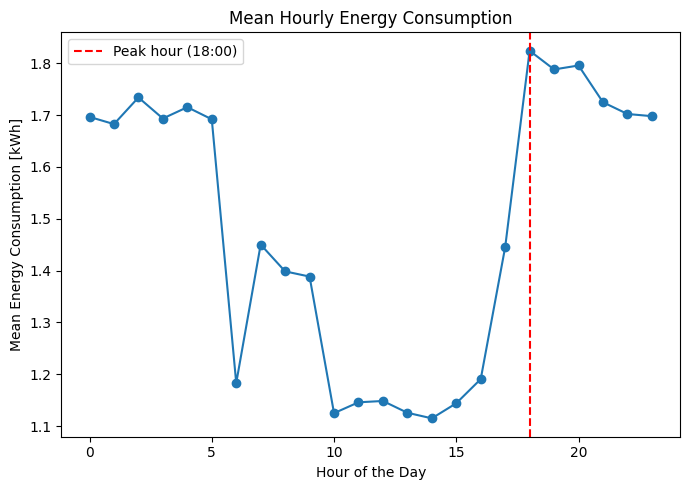
\includegraphics[width=\linewidth]{assets/MeanHourlyConsumption.png}
        \caption{Hourly energy consumption.}
        \label{fig:mean_hourly_energy}
    \end{subfigure}
    \hfill  % horizontal space between subfigures
    \begin{subfigure}[b]{0.48\linewidth}
        \centering
        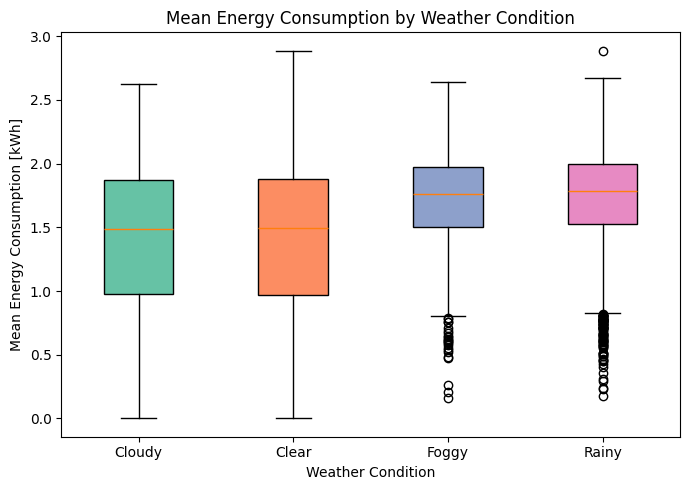
\includegraphics[width=\linewidth]{assets/MeanEnergyByWeather.png}
        \caption{Energy by weather condition.}
        \label{fig:energy_weather}
    \end{subfigure}
    
    \caption{Energy consumption patterns under different temporal and environmental conditions.}
    \label{fig:energy_analysis}
\end{figure}

\subsection{Safety and Special Events}
Energy usage was evaluated with respect to safety risk levels, showing that areas or periods with higher perceived risk were associated with increased lighting. This trend suggests that the system can prioritize safety through dynamic adjustments.

Additionally, mean energy consumption during special events was examined, revealing localized spikes in demand corresponding to increased pedestrian activity. This highlights the importance of incorporating contextual awareness in intelligent lighting control.

\begin{figure}[H]
    \centering
    \begin{subfigure}[b]{0.48\linewidth} 
        \centering
        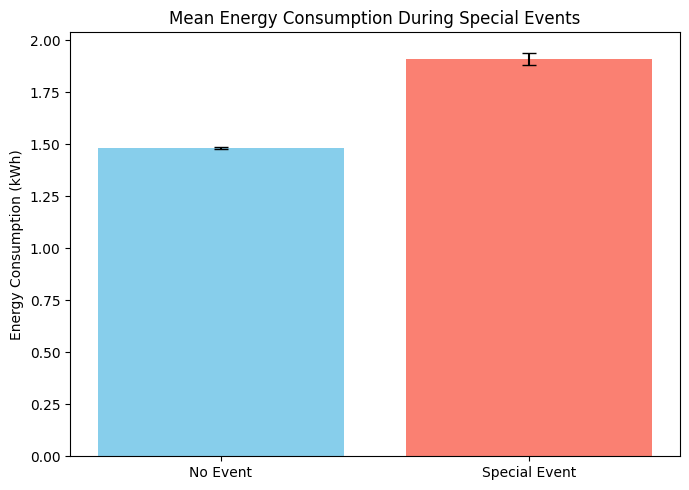
\includegraphics[width=\linewidth]{assets/EnergySpecialEvent.png}
        \caption{During special events.}
        \label{fig:energy_special_event}
    \end{subfigure}
    \hfill
    \begin{subfigure}[b]{0.48\linewidth}
        \centering
        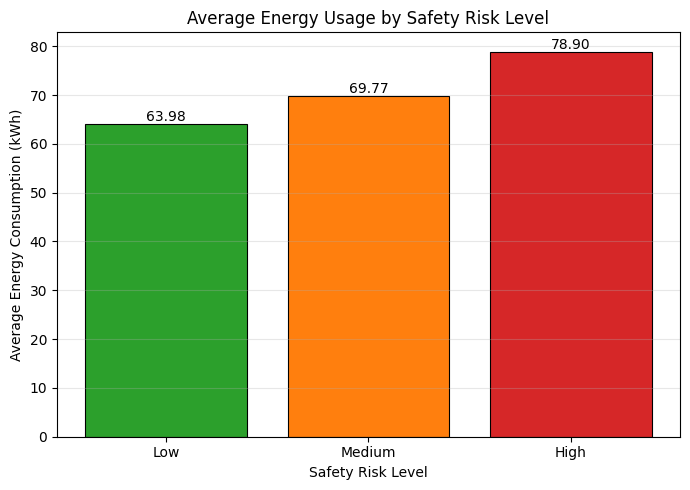
\includegraphics[width=\linewidth]{assets/EnergyvsRisk.png}
        \caption{By safety risk level.}
        \label{fig:energy_vs_safety_risk}
    \end{subfigure}
    
    \caption{Energy consumption patterns under special conditions and varying safety risks.}
    \label{fig:energy_analysis_special_risk}
\end{figure}


\subsection{Density-Level Analysis}

Finally, energy consumption was analysed across traffic density levels categorized as low, medium, and high (Fig.~\ref{fig:energy_traffic_analysis}b). The results show a clear relationship between pedestrian and vehicle density and lighting energy requirements, indicating that density-aware control strategies can further improve energy efficiency while maintaining safety.

\begin{figure}[H]
    \centering
    \begin{subfigure}[b]{0.48\linewidth}
        \centering
        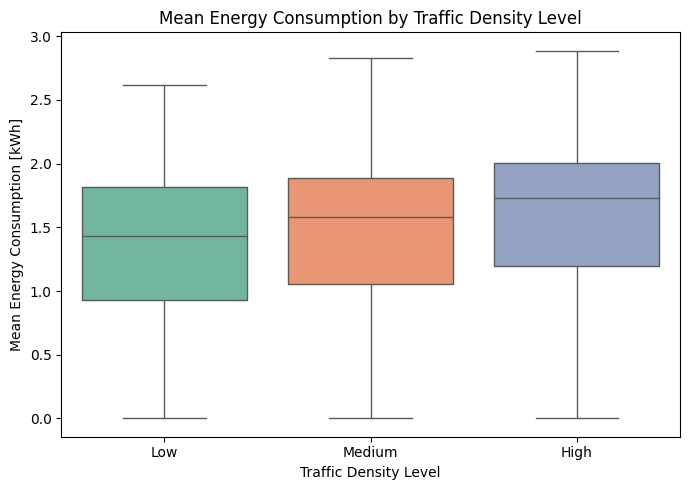
\includegraphics[width=\linewidth]{assets/EnergyByTraffic.png}
        \caption{Energy by traffic level.}
        \label{fig:energy_by_traffic}
    \end{subfigure}
    \hfill
    \begin{subfigure}[b]{0.48\linewidth}
        \centering
        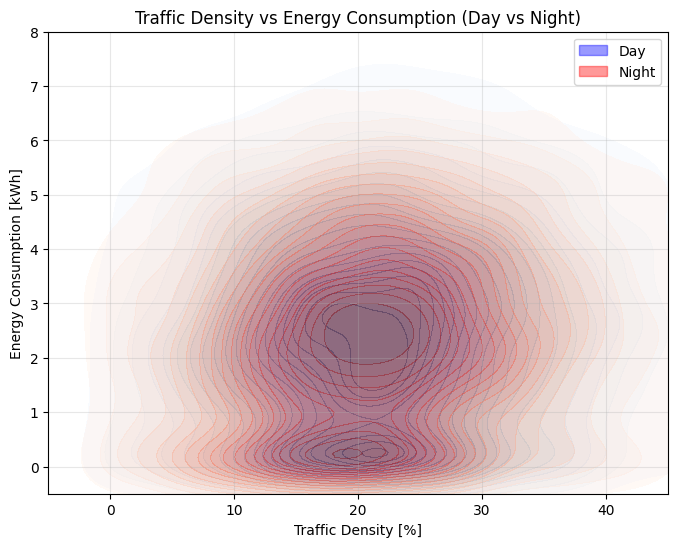
\includegraphics[width=\linewidth]{assets/EnergyvsTrafficDensity.png}
        \caption{Energy vs. traffic density and time.}
        \label{fig:energy_vs_traffic_density}
    \end{subfigure}
    
    \caption{Energy consumption relative to traffic conditions.}
    \label{fig:energy_traffic_analysis}
\end{figure}

\section{Model Results and Interpretation}
\subsection{ML Predictor Performance}

\begin{table}[H]
\centering
\caption{Ranking of Optimizers Based on Predictive Performance}
\label{tab:optimizer_ranking}
    \begin{tabular}{c|l|c|c|c|c}
        \hline
        \textbf{Rank} & \textbf{Optimizer} & \textbf{RMSE} & \textbf{MAE} & \textbf{$R^2$} & \textbf{Runtime (s)} \\
        \hline
        1 & Adam      & \textbf{8.174} & 6.472 & \textbf{0.8672} & 94.47 \\
        2 & Nadam     & 8.176 & \textbf{6.456} & 0.8672 & 97.01 \\
        3 & Momentum  & 8.289 & 6.580 & 0.8635 & 79.79 \\
        4 & RMSprop   & 8.289 & 6.523 & 0.8635 & 86.30 \\
        5 & SGD       & 8.312 & 6.595 & 0.8627 & 173.58 \\
        6 & Lion      & 8.419 & 6.649 & 0.8592 & 80.62 \\
        7 & AMSGrad   & 8.549 & 6.750 & 0.8548 & 117.94 \\
        8 & Adagrad   & 61.638 & 58.181 & -6.5491 & 83.78 \\
        9 & Adadelta  & 67.047 & 63.395 & -7.9322 & 101.94 \\
        \hline
    \end{tabular}
\end{table}

Several gradient-based optimizers were tested, including classical stochastic gradient descent variants and adaptive methods. Performance was evaluated on a held-out test set using RMSE, MAE, and $R^2$ to measure average error, sensitivity to outliers, and overall fit (Table~\ref{tab:optimizer_ranking}).

Adam achieved the best performance (RMSE $=$ 8.174, $R^2 = 0.8672$), making it the preferred optimizer for training the standalone MLP predictor in subsequent experiments. It was followed closely by Nadam, while Momentum and RMSprop formed a second tier with comparable accuracy. SGD showed slightly lower performance and longer runtime, Lion and AMSGrad exhibited moderate degradation, and Adagrad and Adadelta failed to converge, yielding very high RMSE and negative $R^2$ values. This ranking highlights the effectiveness of adaptive moment-based optimizers for learning complex nonlinear relationships in the smart lighting dataset and informed the choice of optimizer for the hybrid control framework.

\subsection{Regression Model Performance}

We compared the standalone MLP predictor with several regression models, including Gradient Boosting, XGBoost, and Random Forest. All models were evaluated, with recorded runtime to assess computational efficiency (Table~\ref{tab:model_ranking}).

\begin{table}[H]
\centering
\caption{Ranking of Regression Models Based on Predictive Performance}
\label{tab:model_ranking}
\begin{tabular}{c|l|c|c|c|c}
\hline
\textbf{Rank} & \textbf{Model} & \textbf{RMSE} & \textbf{MAE} & \textbf{$R^2$} & \textbf{Runtime (s)} \\
\hline
1 & Gradient Boosting & \textbf{$7.2352$} & \textbf{$5.5802$} & \textbf{$0.8960$} & $8.98$ \\
2 & XGBoost & $7.2540$ & $5.6142$ & $0.8954$ & $0.40$\\
3 & Random Forest & $7.2619$ & $5.5807$ & $0.8952$ & $13.73$\\
4 & MLP & $8.1738$ & $6.4718$ & $0.8672$ & $94.47$ \\
5 & Ridge Regression & $8.3420$ & $6.6259$ & $0.8617$ & $0.004$\\
6 & Elastic Net & $8.3474$ & $6.6333$ & $0.8615$ & $0.05$\\
7 & Lasso Regression & $8.3482$ & $6.6333$ & $0.8615$ & $0.08$\\
\hline
\end{tabular}
\end{table}

Gradient Boosting achieved the best overall performance (RMSE $=$ 7.235, $R^2 = 0.896$), narrowly outperforming XGBoost and Random Forest. The standalone MLP performed slightly worse (RMSE $=$ 8.174, $R^2 = 0.867$) and required substantially longer runtime, highlighting the trade-off between model complexity and training cost. Linear models such as Ridge, Elastic Net, and Lasso showed lower predictive accuracy, confirming the need for nonlinear modeling on this dataset.

\subsection{Final Comparison: Standalone MLP vs. Hybrid MLP+Fuzzy Model}
The standalone MLP achieved the highest predictive accuracy, with an RMSE of 8.174, an MAE of 6.456, and an $R^2$ of 0.8672, ranking first when models are evaluated purely on regression performance. These results confirm the neural network’s ability to capture complex nonlinear relationships between environmental conditions, activity levels, and lighting demand.

The hybrid MLP+Fuzzy model exhibited a slightly different performance profile, with an RMSE of 8.162, an MAE of 6.472, and an $R^2$ of 0.858, placing it second in predictive accuracy. The minor reduction in accuracy is expected, as the fuzzy layer deliberately adjusts MLP outputs according to rule-based constraints.

Importantly, the hybrid model prioritizes robustness, interpretability, and safety-aware decision-making over purely minimizing prediction error. By constraining extreme or potentially unsafe outputs, the fuzzy layer enforces conservative lighting adjustments under low visibility or atypical activity. This trade-off results in a small loss of predictive accuracy in exchange for enhanced control reliability, making the hybrid approach better suited for real-world street lighting deployment where safety and explainability are critical.

\section{Results of the Study}
\subsection{Energy Efficiency}

Fig.~\ref{fig:cumulative_energy} and~\ref{fig:energy_window} compare the energy performance of the baseline system driven by raw sensor data with the proposed EA--MLP--Fuzzy optimized strategy, at both cumulative and short-term resolutions. The plot (Fig.~\ref{fig:cumulative_energy}) shows a clear divergence between the two trajectories over the one-year evaluation period, with the optimized approach achieving substantially lower aggregate consumption. On average, this corresponds to an energy saving of \textbf{17.8\%}, highlighting the effectiveness and stability of the optimization framework.

The short-window hourly energy plot (Fig.~\ref{fig:energy_window}) shows the system’s behavior at a finer scale. The optimized strategy usually consumes less energy than the baseline, though occasional short spikes occur due to temporary control actions or load adjustments. Occasional short spikes occur due to temporary control adjustments, but these are outweighed by frequent energy reductions. Overall, the results show that the EA--MLP--Fuzzy approach achieves substantial long-term energy savings while remaining reliable under changing conditions.

\begin{figure}[H]
    \centering
    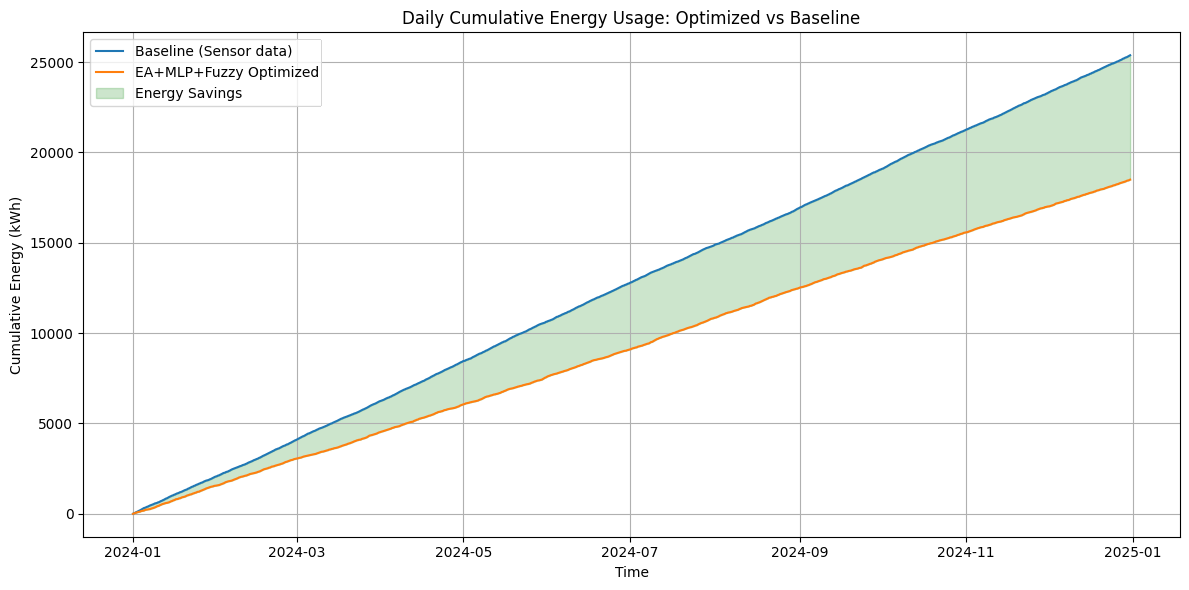
\includegraphics[width=0.75\linewidth]{assets/Results1.png}
    \caption{Daily Cumulative Energy Usage Optimized vs Baseline (Sensor Data)}
    \label{fig:cumulative_energy}
\end{figure}

\begin{figure}[H]
    \centering
    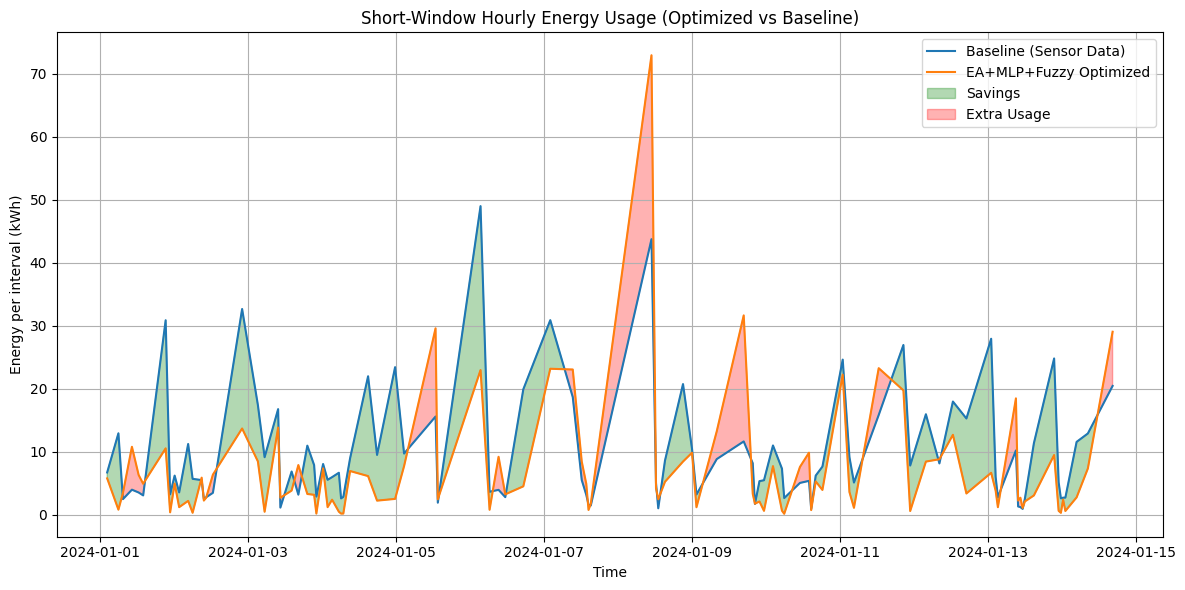
\includegraphics[width=0.75\linewidth]{assets/Results2.png}
    \caption{Short-window hourly energy consumption comparing baseline sensor-driven lighting and EA+MLP+Fuzzy optimized lighting. Green shading indicates energy savings, red indicates slightly higher usage.}
    \label{fig:energy_window}
\end{figure}

\subsection{Safety Assessment}

\begin{figure}[H]
    \centering
    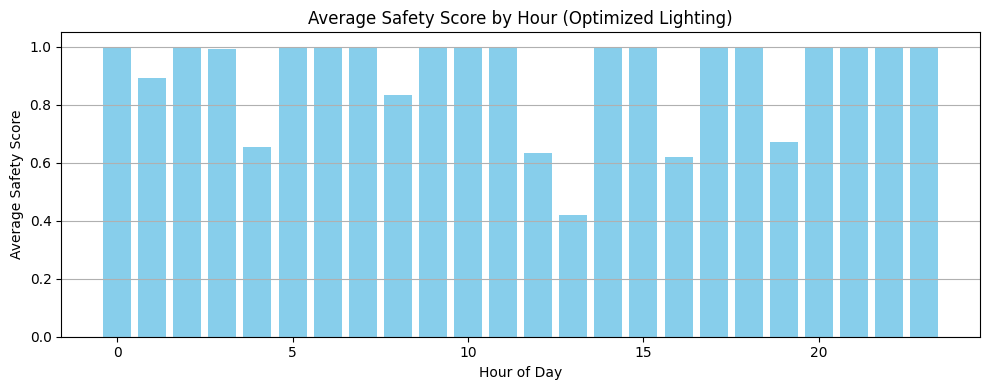
\includegraphics[width=0.75\linewidth]{assets/SafetyPerHourOptimized.png}
    \caption{Average hourly safety score for the optimized lighting system. Shows how safety is maintained across different hours of the day.}
    \label{fig:hourly_safety}
\end{figure}

Safety performance was evaluated using a custom safety score that incorporates environmental visibility and optimized light intensity. Fig.~\ref{fig:hourly_safety} presents the average safety score by hour of day for the optimized system.

\begin{figure}[H]
    \centering
    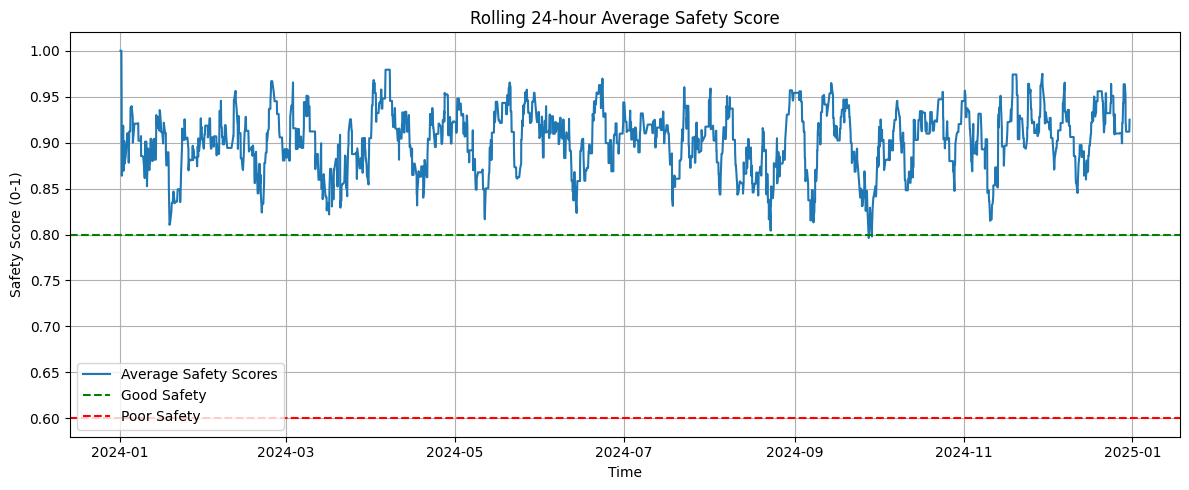
\includegraphics[width=0.8\linewidth]{assets/SafetyScoreInTimeWindow.png}
    \caption{Rolling 24-hour average safety score for the optimized system. Horizontal lines indicate “good” and “poor” safety thresholds.}
    \label{fig:rolling_safety}
\end{figure}

Figure~\ref{fig:rolling_safety} shows the rolling 24-hour average safety score. Horizontal reference lines indicate thresholds for “good” (0.8) and “poor” (0.6) safety levels.

\section{Discussion and Conclusion}

The proposed hybrid smart street lighting system demonstrates strong potential for improving energy efficiency while maintaining public safety. By combining a data-driven MLP predictor, which captures nonlinear relationships in environmental conditions and human activity, with a fuzzy-rule expert layer for safety-aware decision-making, the framework balances adaptive illumination and energy conservation. This design reduces unnecessary power consumption during low-demand periods while ensuring adequate lighting under uncertain conditions.

The evaluation highlights that the hybrid approach mitigates extreme predictions from the standalone MLP, providing robustness and interpretability. Consistent energy savings across varying traffic, occupancy, and environmental conditions illustrate the benefit of integrating predictive intelligence with rule-based reasoning. The modular architecture also allows future expansion to additional sensors, zones, or control objectives without major redesign.

Future work would focus on integrating real-world sensor data and automating fuzzy rule tuning via evolutionary or multi-objective optimization. Extending the framework to city-wide coordination or additional objectives such as user comfort could further enhance performance and scalability.

Overall, hybrid AI combining predictive modeling with interpretable reasoning offers a scalable, transparent, and responsible approach for sustainable smart city infrastructure, delivering energy savings and enhanced safety.

\bibliographystyle{IEEEtran}
\begin{thebibliography}{99}

\bibitem{smartlighting_dataset}
IoT-Enabled Smart Lighting Dataset, Kaggle. [Online]. Available: \url{https://www.kaggle.com/datasets/ziya07/iot-enabled-smart-lighting-dataset}. Accessed: Jan. 14, 2026.

\bibitem{zadeh1965fuzzy}
L. A. Zadeh, ``Fuzzy sets,'' \emph{Information and Control}, vol. 8, no. 3, pp. 338--353, 1965.

\bibitem{ross2010fuzzy}
T. J. Ross, \emph{Fuzzy Logic with Engineering Applications}, 3rd ed. Hoboken, NJ, USA: Wiley, 2010.

\bibitem{holland1992genetic}
J. H. Holland, ``Genetic algorithms,'' \emph{Scientific American}, vol. 267, no. 1, pp. 66--73, 1992.

\bibitem{kingma2015adam}
D. P. Kingma and J. Ba, ``Adam: A method for stochastic optimization,'' in \emph{Proc. Int. Conf. Learn. Representations (ICLR)}, 2015.

\bibitem{wilcoxon1945individual}
F. Wilcoxon, ``Individual comparisons by ranking methods,'' \emph{Biometrics Bulletin}, vol. 1, no. 6, pp. 80--83, 1945.

\bibitem{molina2018smartlighting}
M. Molina \emph{et al.}, ``Smart street lighting systems using machine learning techniques,'' \emph{IEEE Trans. Intell. Transp. Syst.}, vol. 19, no. 5, pp. 1421--1430, May 2018.

\end{thebibliography}

\end{document}